\section{Methodology}

\lstset{
  basicstyle=\small\ttfamily,
  captionpos=b,
  frame=single,
  breaklines=true,
  showstringspaces=false,
  aboveskip=2.5pt,
  belowskip=2pt
}

\subsection{Dataset description}
In this case, the dataset consists of a collection of text messages paired with the corresponding class labels after preprocessing, which can diffuse from each dataset.
Table III shows the structure of the dataset, serving as an illustrative example.
It is important to note that the training is not based on this example data, see Table III.
Various datasets with diverse data will be employed subsequently, making Table III a representative instance rather than an exhaustive depiction of the training process.

\begin{table}[htp]
  \begin{center}
  \label{dataset}
  \caption{Dataset}
  \small
  \begin{tabularx}{\columnwidth}{| X | c |}
          \hline
          Text & Class \\
          \hline
          Hey, how's it going? & Not spam \\
          \hline
          Pay now, or your account will be locked! & Spam \\
          \hline
          Congratulations! You have won a free vacation! & Spam \\
          \hline
          Have a great day! & Not spam \\
          \hline
          ... & ... \\
          \hline
      \end{tabularx}
  \end{center}
\end{table}

\subsection{Model architecture}
\indent The model's code in figure 1 followed a feedforward architecture with three fully connected layers.
These layers, denoted as $fc1$, $fc2$, and $fc3$, were responsible for the linear transformation [3] of the input data.
The first layer processes the input features and the subsequent layers extract hierarchical representations, leading to the final output layer. \\

\indent Rectified Linear Units ($ReLU$) [4] serve as activation functions applied after the linear transformations in the first and second layers.
To prevent overfitting, a dropout [5] layer was strategically placed after each Rectified Linear Unit ($ReLU$) activation step.
This layer randomly sets a fraction of the output units to zero during training, ensuring that the network generalizes well to the unseen data. \\

\indent The output of the model, which represents the likelihood of spam or non-spam for binary classification, is produced by the final layer $fc3$, without any activation function applied to it.

\begin{figure}[htp]
  \begin{lstlisting}[language=Python, label=modell]
    class SpamClassifier(nn.Module):
      def __init__(self, input_dim, hidden_dim1, hidden_dim2, output_dim, dropout_prob):
          super(SpamClassifier, self).__init__()
          self.fc1 = nn.Linear(input_dim, hidden_dim1)
          self.fc2 = nn.Linear(hidden_dim1, hidden_dim2)
          self.fc3 = nn.Linear(hidden_dim2, output_dim)
          self.dropout = nn.Dropout(p=dropout_prob)

      def forward(self, x):
          x = F.relu(self.fc1(x))
          x = self.dropout(x)
          x = F.relu(self.fc2(x))
          x = self.dropout(x)
          x = self.fc3(x)
          return x
  \end{lstlisting}
  \caption{PyTorch code of the model architecture}
\end{figure}

\subsection{Used parameters}
\indent For hidden dimension one, set to 64, this parameter determines the number of neurons in the first hidden layer of the neural network.
For hidden dimension two, we assigned a value of 32, which defines the number of neurons in the second hidden layer.
This layer builds on the representations learned by the first layer and extracts additional features from the data.
Output dimension configured as 2, which defines the number of classes in the classification task.
With a dropout probability of 0.5, dropout layers are incorporated after each activation function to mitigate overfitting.
To achieve improved accuracy, the optimal number of epochs may vary for each dataset.
The choice of epochs balances the training in time with the convergence of the model to a stable state.
The test size, set to 0.2, determines the proportion of the dataset reserved for testing the model's performance. A test size of 0.2 implies that 20\% of the data is held out for evaluation, while the remaining 80\% is used for training.
The learning rate specified as 0.001, governs the step size in the gradient descent optimization process.

\begin{figure}[htp]
    \centering
    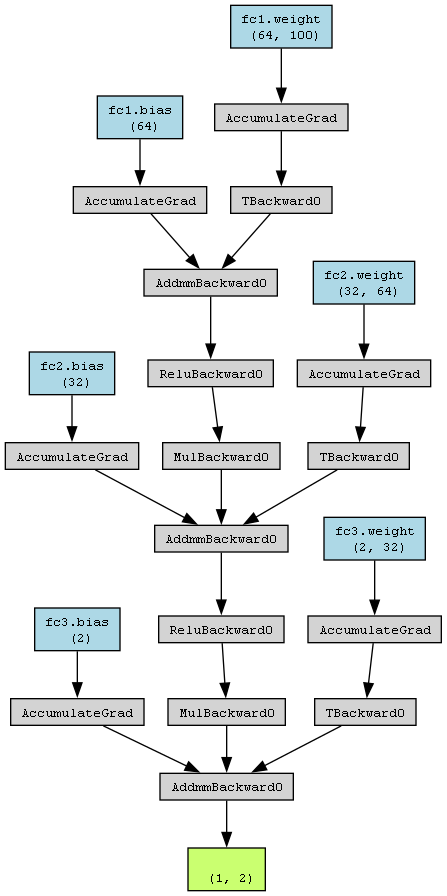
\includegraphics[width=0.4\textwidth]{text_classifier_model.png}
    \caption{Visualization of the model}
\end{figure}

\subsection{Training process}
Figure 2 shows an example input dimension (100) to present the entire training process using the model discussed previously. It is noteworthy that the input dimensions can differ for each dataset. \\

\indent The Cross Entropy Loss ($nn.CrossEntropyLoss()$ as shown in figure 1 was employed [8].
This loss function is well-suited for multi-class classification tasks, providing a measure of the disparity between predicted class probabilities and the true distribution of classes. \\

\indent The Adam optimizer ($optim.Adam$ as shown in figure 1 is selected for its adaptive learning rate properties [9]. \\
Adam is expected to navigate the model parameters effectively during the training process. \\

True Positives (TP):
\begin{itemize}
  \item Cases that were positive (spam) and correctly predicted by the filter were positive (spam).
  \item Example: An email containing known spam keywords and characteristics is correctly classified as spam by the filter.
\end{itemize}

True Negatives (TN):
\begin{itemize}
  \item Cases that were indeed negative (not spam), and the filter correctly flagged them as negative (not spam).
  \item Example: A regular non-spam email, without any spam-like attributes, is correctly identified as not spam by the filter.
\end{itemize}

False Positives (FP):
\begin{itemize}
  \item Cases that were negative (not spam) but wrongly flagged by the filter as positive (spam).
  \item Example: A legitimate email from a friend contains certain words or patterns that the spam filter misclassifies as spam.
\end{itemize}

False Negatives (FN):
\begin{itemize}
  \item Cases that were actually positive (spam) but the filter incorrectly flagged them as negative (not spam).
  \item Example: An actual spam email manages to evade detection and is incorrectly classified as a non-spam email.
\end{itemize}

% \begin{figure}[htp]
%     \centering
%     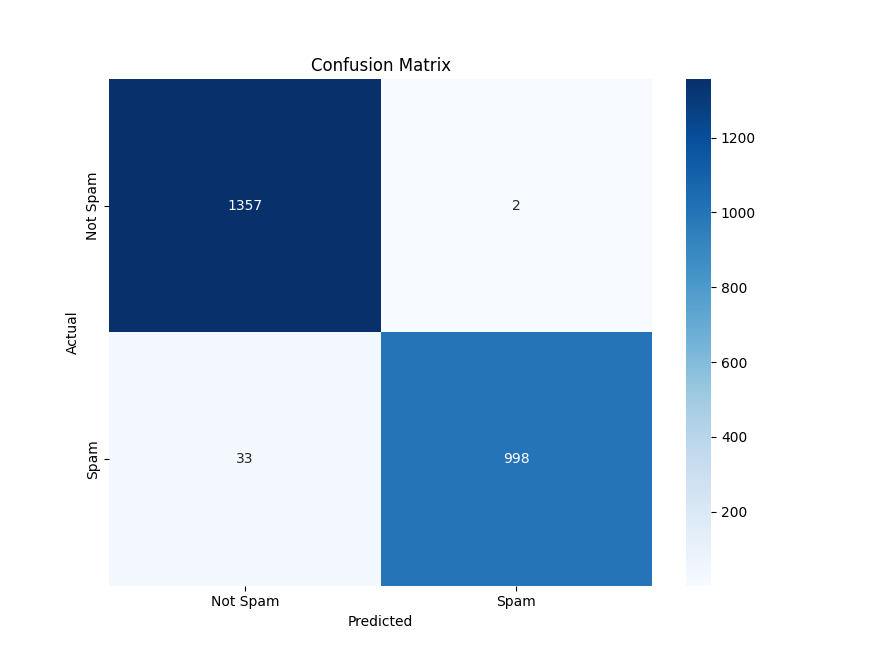
\includegraphics[width=1.1\columnwidth]{confusion_matrix.png}
%     \caption{Confusion Matrix}
% \end{figure}
% \indent The confusion matrix provides a visual representation of these variables, thus making the representation of these values clearer.

% \begin{figure}[htp]
%     \centering
%     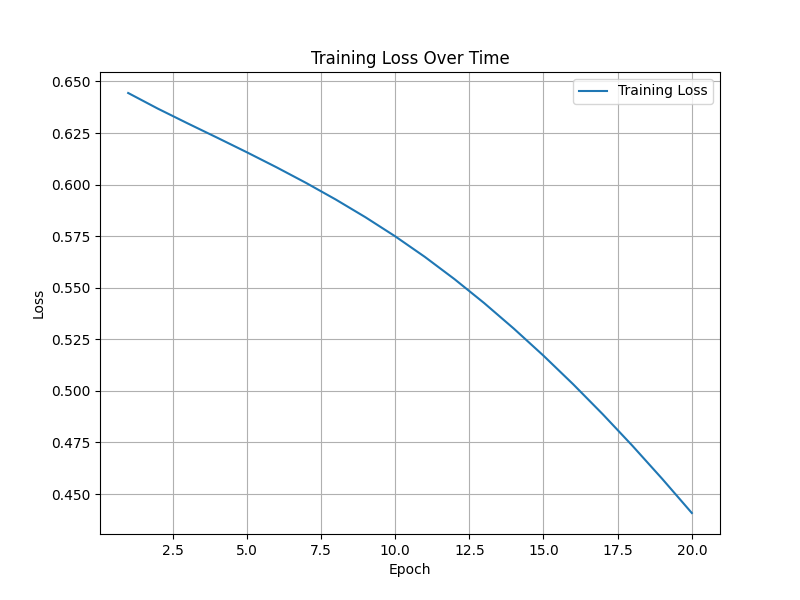
\includegraphics[width=1.1\columnwidth]{training_loss.png}
%     \caption{Training loss over time}
% \end{figure}

\subsection{Evaluation metrics}

These mathematical formulas shows how the accuracy, precision, recall (sensitivity) and f1 score are calculated [6].

\[
  \text{Accuracy} = \frac{TP + TN}{TP + TN + FP + FN}
\]
\indent Accuracy measures the overall correctness of the model by calculating the proportion of correctly predicted cases (true positives and true negatives) relative to all cases.

\[
  \text{Precision} = \frac{TP}{TP + FP}
\]
\indent Precision is the ratio of correctly predicted positive observations (true positives) to the total number of predicted positives. It focuses on how many of the predicted positive cases were actually positive.

\[
  \text{Recall (Sensitivity)} = \frac{TP}{TP + FN}
\]
\indent The recall calculates the ratio of correctly predicted positive observations (true positives) to the total number of true positives. This shows how well the model captures all positive cases.

\[
  \text{F1 score} = 2 \times \frac{Precision \times Recall}{Precision + Recall}
\]
\indent The F1 score is the harmonic mean of accuracy and recall. It balances accuracy and recall and provides a single metric for evaluating model performance. It is particularly useful when the distribution of classes is uneven.